\documentclass[11pt, oneside]{article}   	% use "amsart" instead of "article" for AMSLaTeX format
\usepackage[margin=0.75in]{geometry}                		% See geometry.pdf to learn the layout options. There are lots.
\geometry{letterpaper}                   		% ... or a4paper or a5paper or ... 
%\geometry{landscape}                		% Activate for rotated page geometry
%\usepackage[parfill]{parskip}    		% Activate to begin paragraphs with an empty line rather than an indent
\usepackage{graphicx}				% Use pdf, png, jpg, or eps§ with pdflatex; use eps in DVI mode
\graphicspath{ {Figures/} }								% TeX will automatically convert eps --> pdf in pdflatex		
\usepackage{amssymb}
\usepackage[english]{babel}
\usepackage{csquotes}

\usepackage[backend=biber]{biblatex}
\addbibresource{basic.bib}

%SetFonts

%SetFonts


\title{Deep IV GWAS: Milestone \\
	\large Category: Health / Genomics}
\author{
	Jack Andraka\\ 
	\texttt{jandraka@stanford.edu}
	\and
	Billy Ferguson\\
	\texttt{billyf@stanford.edu}
	\and
	Charlie Walker\\
	\texttt{cwalker4@stanford.edu}
}
\date{}							% Activate to display a given date or no date

\begin{document}
\maketitle
\section{Introduction}
@jandraka 
 The genome-wide association study (GWAS) is an experimental design used to detect associations between genetic variants and traits in samples from populations and has served as a main driver of understanding the relationship between gene expression and phenotype.\textsuperscript{[2,3]} However, since traditional GWAS study designs run several thousand to million t-tests simultaneously they can only identify gene variants with large effect size. This is in contrast with the current hypothesis of genetic architecture that posits many gene variants acting in tandem to produce a phenotypic trait, each with small effect size.\textsuperscript{[4]} \\
 
 Despite the development of many sophisticated modern statistical techniques to deal with complicated interactions like the ones between genes, GWAS is plagued by counfoundedness. Gene expression and phenotype directly influence each other, rendering simple prediction or correlations between the two useless. While neural networks seem to provide the best ability to uncover complicated interactions between genes, they are not built to parse through endogeneity.  To address these shortcomings we will employ the Deep IV methodology, a two-stage multiplayer perceptron model designed to use exogenous instruments $z$ to identify the direct causal relationship of some policy variable $p$ on outcome $y$. In our case, we want to use random gene mutations to characterize the causal effect of gene expression on phenotype.\\
 
 @jandaraka Write about why this is such a big deal for GWAS and then why GWAS is such a big deal. 

\section{Algorithm}
\subsection{Overview}
We implement the method described in ``Deep IV: A Flexible Approach for Counterfactual Prediction'' to identify the effect of a policy variable $p$ on outcome $y$ under confoundedness.\textsuperscript{[5]} Instrumental variables (IV) are a well-developed tool for remedying endogeneity, but require a strong prior understanding of the data generating process and are not well equipped to deal with a large number of covariates. Deep IV promises to marry the best qualities of DNNs and IV, and we believe GWAS are a prime use case. \\

To perform IV analysis one needs to find an exogenous variable that affects the outcome variable only through the endogenous covariate of interest. More specifically, the instrument \emph{z} must be conditionally independent of the error (Figure 1).\\

\begin{figure}[h]
	\caption{Generalized Deep IV}
	\centering
	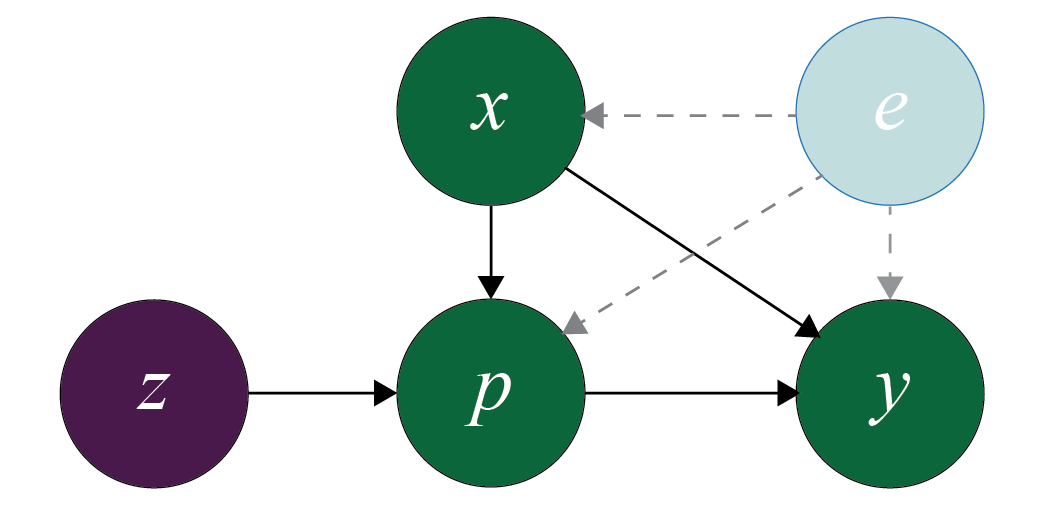
\includegraphics[width=0.6\textwidth]{Figure_1.png}
\end{figure}

Traditional IV can be estimated through a procedure called two-stage least squares (2SLS): in the first stage you regress your endogenous variable of interest, $p$,  on the exogenous instrument, $z$, to create a predicted $\hat{p}$ constructed only with the exogenous variation of $z$. In the second stage, you regress your outcome variable, $y$, on the predicted $\hat{p}$ from the first stage.\footnote{Chapter 4 of Angrist and Pischke's \emph{Mostly Harmless Econometrics: an Empiricist's Companion} provides a good introduction to instrumental variables.}\\

\subsection{Model Architectures}

To adapt this procedure for the DeepIV method, we replace the two-stage least squares with two-stage multilayer perceptrons. We call the first stage our \emph{policy network} and the second our \emph{response network}. Our first iteration is modeled off of the specification in the appendix of the seminal DeepIV paper from Hartford et al. (2017).\textsuperscript{[6]}\\

The policy and response networks have three hidden layers with 128, 64, and 32 hidden units respectively. The policy network takes in the exogenous $z$ and control variables $x$ as input to predict $p$ using tanh acitvation functions for each layer and a mixture of Gaussian output with 10 components. The predicted $\hat{p}$ from the policy network and $x$ are then fed into the response network to yield predictions $\hat{y}$. The repsone network performs ReLU activation functions for the three hidden layers and linear activation for the output. \\

Both networks use Adam Optimization with learning rate $=.001$, $\beta_1 = .9$, $\beta_2 = .999$, and $\epsilon = 1e-08$. For training we use L2 regularized weight decay set to $0.001$, a dropout rate of $min(1000/(1000+n); 0.5)$, $(1.5 \times 10^6/n)$ epochs, and batch size $100$. 


\section{Experiment}
\subsection{Motivation and Design}
What is the simulated data and why are we doing it @cwalker4

\subsection{Preliminary Results} 
Results of @billyf and @cwalker4 simulations.

\section{Data}
@jandraka

\section{Next Steps}
@jandraka 


\end{document}  